\section{The Gatekeeper Role}\label{sec:gatekeeper}
Gatekeepers are critical to the Gateway Protocol’s operation. They provide the compliance, KYC, or identity verification service that dApps need to ensure they comply with any appropriate rules or regulations in their sector or geographic area.

Each Gatekeeper belongs to one or more Gatekeeper networks and completes User verification in line with these networks’ Governance frameworks. It is this verification that enables dApps to transact with users while fulfilling two needs:

\begin{enumerate}
\item Ensuring the User is legally eligible to enter into the transaction; and,
\item Maintaining the User’s privacy.
\end{enumerate}

\begin{figure}[h]
  \begin{center}
    \centering
    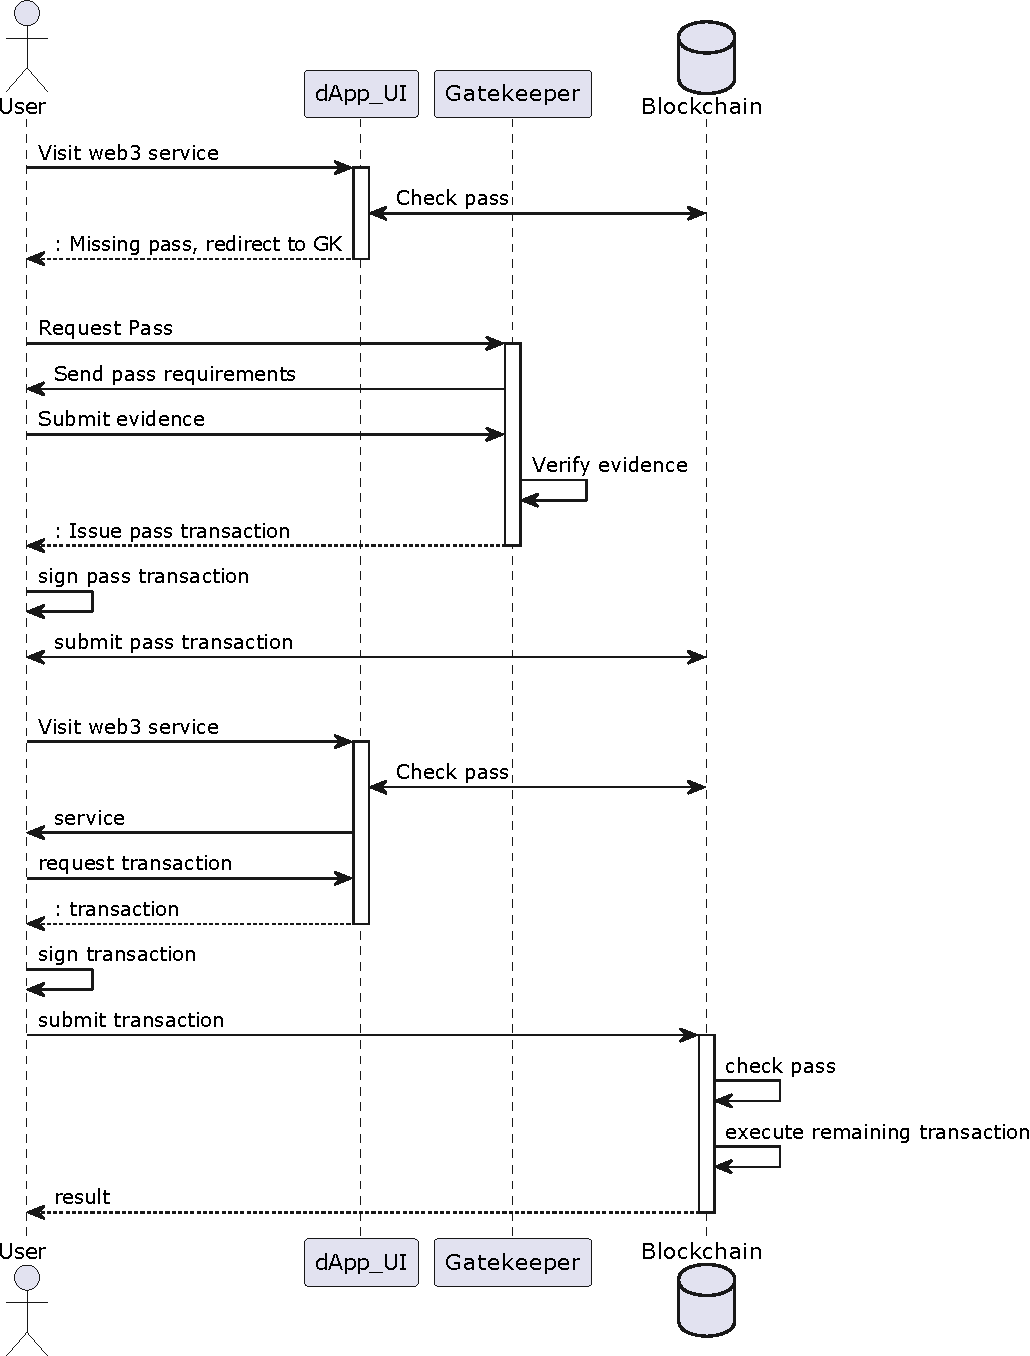
\includegraphics[width=100mm,scale=0.5]{figures/04-sequence-diagram.pdf}
    \caption{Sequence diagram for obtaining a Gateway pass from a Gatekeeper and verifying it within a dApp application}
  \end{center}
\end{figure}

Simply, Gatekeepers removes the burden of KYC/compliance verification from the dApp, so it can transact with users with confidence without reviewing or holding any personal data.

Gatekeepers are also key players in the governance of Gatekeeper networks.

\subsection{What is a Gatekeeper?}
A gatekeeper is a legal entity that enables the Gateway Protocol by completing compliance/KYC checks on users. When a Gatekeeper successfully verifies a User’s compliance with an appropriate Gatekeeper network’s framework, it issues the User with a Gateway Pass.

Gatekeepers operate as oracles that bridge the trust layer between off-chain credential trust—and possibly other verification requirements not directly related to credentials—and the on-chain dApps that require the trusted information to be part of a permissioned Pass.

Most Gatekeepers will likely be organizations that already have KYC and identity verification capabilities for use in traditional financial transactions. The Guardian will regularly audit Gatekeepers to ensure these capabilities are robust and repeatable and remain so over time.
The Guardian will also ensure Gatekeepers adhere to the requirements set by any networks they participate in, which may change over time.

\subsection{Becoming a Gatekeeper}

To become a Gatekeeper within a Gatekeeper network, an organization must go through four steps:

\begin{enumerate}
\item Ensure it has the necessary capabilities to complete appropriate User verifications for a specific Gatekeeper network.
\item Apply to join the Gatekeeper network.
\item Undergo an audit by the Guardian to ensure the necessary capabilities are in place. Audits may also be completed by an authorized third party authorized by the Guardian, e.g., an external accounting firm.
\item Stake a specified minimum amount of Governance Tokens, determined by the volume of Gateway Pass operations they will perform.
\end{enumerate}

Once these four steps are completed, the organization joins the desired Gateway network(s) and can begin offering its verification services to users.

\subsection{Staking}

Staking Governance Tokens will be a requirement for becoming and remaining a Gatekeeper. The stake will incentivize Gatekeepers to uphold their duties and act in the best interest of the Gateway Protocol. There will also be regular Gateway Protocol network fee for Gatekeepers to pay towards the network, which will automatically be taken from existing Gatekeeper stakes.
These fees are used to fund further protocol development and pay Guardians for their supervisory services.

Each Gatekeeper’s Stake exists to ensure the Gatekeeper’s:

\begin{itemize}
\item Service delivery uptime.
\item Proper operation, i.e., only issuing Gateway Passes in line with the relevant Gatekeeper network’s Governance framework.
\item Adherence to Gatekeeper network rules, i.e., maintaining the capabilities needed to be a Gatekeeper within a network.
\item Thorough documentation of operations within the Protocol.
\end{itemize}

The Guardian will have the power to slash the stake of any Gatekeeper that fails to uphold its duties. Examples of infringements that could result in stake slashing include:

\begin{itemize}
\item Falling below a minimum established service delivery uptime.
\item Issuing Gateway Passes to users who do not meet the requirements of a network.
\item Not keeping appropriate records and documentation.
\item Failing audits and/or not remedying audit failures promptly.
\end{itemize}

If a Gatekeeper repeatedly fails to uphold its duties or commits a serious infraction, the Guardian has the power to remove it from the Protocol and slash its outstanding stake.

Gatekeeper Stakes are global and not associated with any specific Gatekeeper network. The required Stake for Gatekeepers is calculated based on the number of Gatekeeper networks they are in and the Gateway Pass Utilization they generate within a specified time frame.
